\documentclass{article}

% \articletype{inv} % article type

\usepackage[margin = 1in]{geometry}

\usepackage[style=authoryear,natbib=true]{biblatex}
\bibliography{../../bibtex/10_Aim1.bib}

\usepackage{amsmath}
\usepackage{bm}
\usepackage{tabu}
\usepackage{graphicx}
\usepackage{caption}
\usepackage{subcaption}

\newcommand{\T}{^\text{T}}
\newcommand{\N}{\text{N}}
\newcommand{\twolinecell}[2][c]{%
  \begin{tabular}[#1]{@{}c@{}}#2\end{tabular}}
\graphicspath{{images/}}

\newcommand{\redstar}{\textcolor{red}{*}}


\title{\texttt{vqtl}: An \texttt{R} package for Mean-Variance QTL Mapping}
\author{Robert W. Corty and William Valdar}
% \author[$\ast$]{Robert W. Corty}
% \author[$\ast, 1$]{William Valdar}
% \affil[$\ast$]{Department of Genetics, University of North Carolina at Chapel Hill}


% \keywords{QTL mapping, variance heterogeneity}
% \runningtitle{R package mvqtl} % For use in the footer
% \correspondingauthor{Robert Corty}
% \setboolean{displaycopyright}{true}


\begin{document}

\maketitle
% \thispagestyle{firststyle}
% \logomark
% \articletypemark
% \marginmark
% \firstpagefootnote
% \correspondingauthoraffiliation{Correspondence e-mail: william.valdar@unc.edu}
% \vspace{-11pt}%


\begin{abstract}
Most existing methods for QTL mapping in experimental crosses assume that the residual variance is constant across all individuals.
But common situations violate this assumption.
For many phenotypes, one sex is more variable than the other, some experimenters make more precise measurements than others, and specific genetic factors influence environmental sensitivity.
In these cases, mean-variance QTL mapping provides higher power and better protection against false positives.
It also allows for detection of QTL that influence phenotype variance, termed vQTL and QTL that influence some mixture of phenotype mean and variance, termed mvQTL.

We present \texttt{R} package \texttt{vqtl}.
This package makes it easy for geneticists to apply the mean-variance QTL mapping approach, control family-wide error rate (FWER), and visualize and interpret their results.
Because this package is interoperable with the popular \texttt{R/qtl} package and uses many of the same data structures and input patterns, it will be easy for geneticists to analyze future experiments with \texttt{R/vqtl} as well as re-analyze past experiments, possibly discovering new QTL.
\end{abstract}



\section*{Introduction}

QTL mapping studies have provided important insights on nearly every trait of interest in human health and disease.
Advances in breeding, phenotyping \citep{Yang2014a}, and genotyping \citep{Williams1990} model organisms as well as statistical methods \citep{Lander1989a} and software tools \citep{Broman2003} have supported these discoveries.

One common assumption in the design and analysis of these studies is that, across all organisms in a study population, the residual variance is constant.
Said another way, it is typically assumed that nothing -- neither environmental factors nor genetic factors -- influences the residual variance of the trait.

% In fact, gene-gene interactions, gene-environment interactions, genetic factors that influence microenvironmental sensitivity, and environmental factors can influence residual variance.


``vQTL'' analysis challenges that assumption by seeking to identify genetic factors that influence the extent of residual variation \citep{Ronnegard2011a,Ronnegard2012,Cao2014}.
In the companion pieces, we describe an elaboration of ``vQTL'' analysis, the mean-variance QTL mapping approach and use it to discover new QTL from existing data resources [companion B, C].
% This approach allows for QTL mapping in the presence of both genetic and non-genetic effects on phenotype mean and variance.
% We compare its behavior to other QTL mapping approaches, and illustrate the discovery of a new QTL from an existing study.

In support of other researchers who may be interested in mvQTL mapping, we created \texttt{R} package \texttt{vqtl}, which provides functions for conducting genome scans, assessing the statistical significance of results, and visualizing and interpreting significant findings.
\texttt{R} package \texttt{vqtl} uses the same \texttt{cross} data structure as the popular \texttt{qtl} package and is available on \texttt{CRAN}, so it is easy to get started.

Here, we demonstrate typical use of the \texttt{vqtl} package.
The code used to simulate the phenotypes, calculate the statistics, estimate their significance, and visualize significant results is available at \texttt{github.com/rcorty}.



\section*{Simulation of an Illustrative Dataset}

We used the popular \texttt{R/qtl} package to simulate an example experimental cross.
This cross consisted of 200 male and 200 female F2 offspring, with 3 chromosomes of length 100 cM, each tagged by 11 equally-spaced markers and estimated genotype probabilities at 2cM intervals with \texttt{R/qtl}'s hidden Markov model.

We simulated four phenotypes:

\begin{enumerate}
	\item \texttt{phenotype1} consists only of random noise and will serve as an example of negative results for all tests.
	\item \texttt{phenotype2} is influenced by the 6th (middle) marker on chromosome one.  The marker influences the mean of the phenotype, but not the variance, so it will serve as an example of a pure ``mQTL''.
	\item \texttt{phenotype3} is influenced by the 6th (middle) marker on chromosome two.  The marker influences the variance of the phenotype, but not the mean, so it will serve as an example of a pure ``vQTL''.
	\item \texttt{phenotype4} is influenced by the 6th (middle) marker on chromosome three.  The marker influences both the mean and the variance of the phenotype, so it will serve as an example of a mixed ``mvQTL''.
\end{enumerate}

We additionally consider \texttt{phenotype1x} through \texttt{phenotype4x}, which have the same type of genetic effects as \texttt{phenotype1} through \texttt{phenotype4}, but additionally have covariate effects on phenotype variance.
All the same analyses and plots that are shown for \texttt{phenotype1} through \texttt{phenotype4} are shown for \texttt{phenotype1x} through \texttt{phenotype4x} in the appendix.




\section*{Genome Scans}

\begin{figure}[t]
    \begin{subfigure}[b]{0.9\textwidth}
        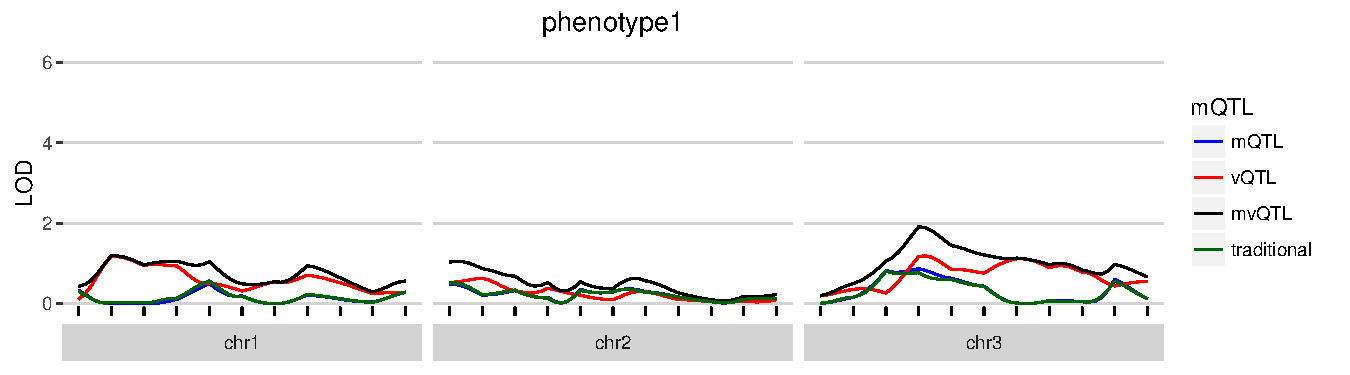
\includegraphics[width=\textwidth]{images/LOD_scan_phenotype1.pdf}
    \end{subfigure}
    \begin{subfigure}[b]{0.9\textwidth}
        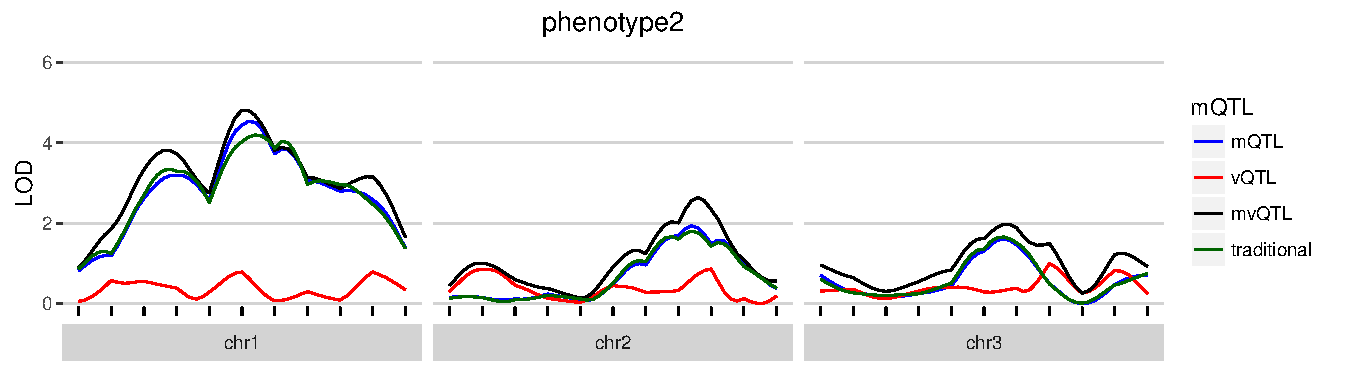
\includegraphics[width=\textwidth]{images/LOD_scan_phenotype2.pdf}
    \end{subfigure}
    \begin{subfigure}[b]{0.9\textwidth}
        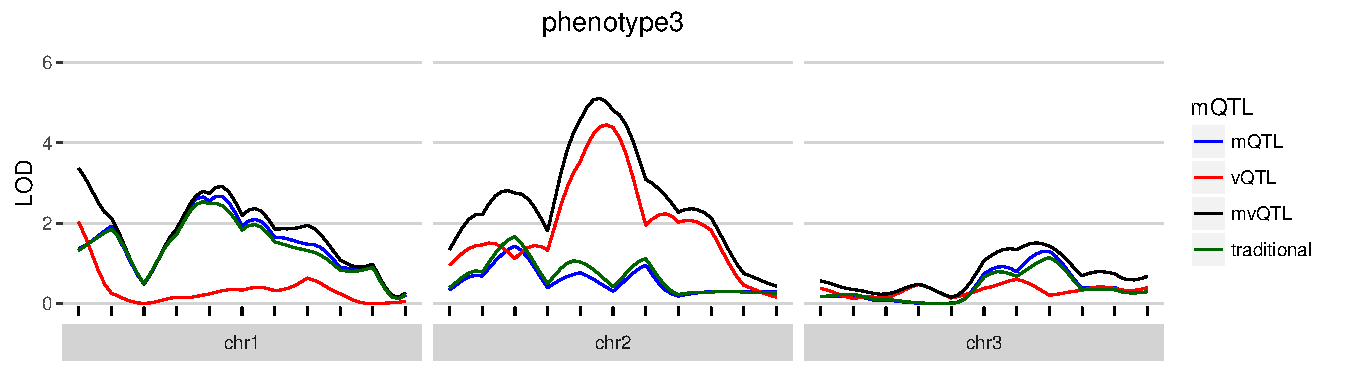
\includegraphics[width=\textwidth]{images/LOD_scan_phenotype3.pdf}
    \end{subfigure}
    \begin{subfigure}[b]{0.9\textwidth}
        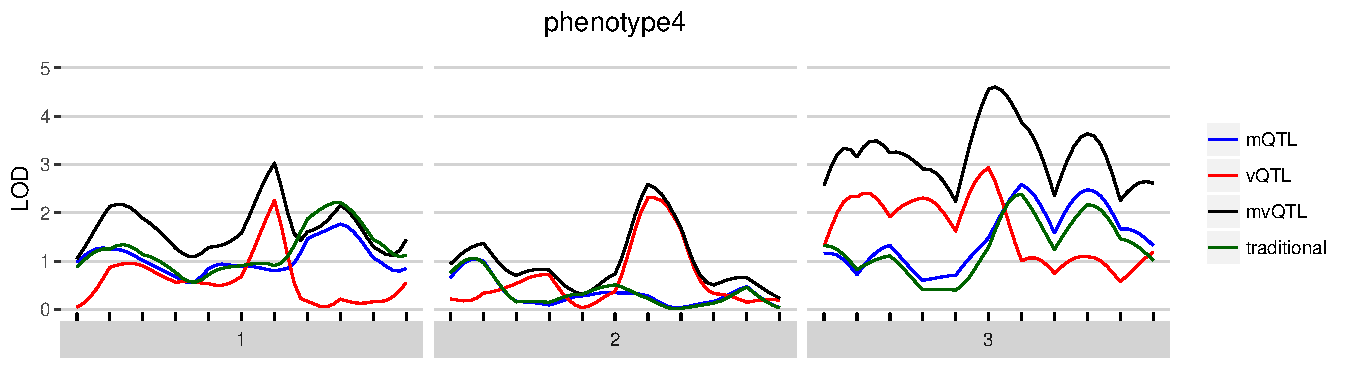
\includegraphics[width=\textwidth]{images/LOD_scan_phenotype4.pdf}
    \end{subfigure}
    \caption{For each of the four simulated phenotypes, the genome scan shows the LOD score of each test -- mean, variance, and joint -- in blue, red, and black, respectively.  The traditional test is in green and globally similar to the mean test. \label{fig:lod_score_scans}}
\end{figure}

The central function for genetic mapping in package \texttt{qtl} is \texttt{scanone} \citep{Broman2003}.
Analogously, the central function for genetic mapping in package \texttt{mvqtl} is \texttt{scanonevar}.
It takes three required inputs:

\begin{enumerate}
    \item \texttt{cross} contains the genetic and phenotypic information from an exerimental cross.  This object can be the same \texttt{cross} object used in package \texttt{qtl}.
    \item \texttt{mean.formula} specifies the phenotype to be mapped, the covariates to be corrected for, and the QTL terms to be fitted (\texttt{additive} and \texttt{dominance} components by default).  The \texttt{mean.formula} uses the standard \texttt{R} formula notation.
    \item \texttt{var.formula} specifies the covariates to be corrected for as well as the QTL terms to be fitted (\texttt{additive} and \texttt{dominance} components by default) in modeling the residual variance.  The \texttt{var.formula} also uses the standard \texttt{R} formula notation.
\end{enumerate}

Optional argument \texttt{chrs} is used to specify a subset of chromosomes to be scanned, defaulting to all chromosomes.
Optional argument \texttt{return.covar.effects} is used to specify whether or not fitted effects of all covariates should be returned as part of the scan result, defaulting to \texttt{FALSE}.
This option can be useful in assessing the trends in the various genetic components of the phenotype across the genome or in assessing the trends in covariate effects across the genome.

Unlike \texttt{scanone}, which only tests for association between each locus and the phenotype mean, \texttt{scanonevar} computes three tests for each locus -- association with phenotype mean, association with phenotype variance, and joint association with phenotype mean and variance.
The statistic for each of these associations is a LOD score, a the log of the ratio of the likelihood of the alternative model to the null model.
The results of \texttt{scanonevar} on each of the four described phenotypes is shown in figure~\ref{fig:lod_score_scans}.
The details of the null and alternative models used in each of the three tests can be found in the companion article [Corty2017a, Corty2017b].


\subsection*{The LOD Score -- Problems and an Alternative}
The traditional test statistic in QTL mapping is the LOD score, but its interpretation can be difficult for two reasons:
(1) LOD scores must be interpreted differently in autosomes and sex chromosomes.
The sex chromosomes are typically fit with fewer parameters, depressing the expected value of the LOD scores under the null, and thus increasing the significance of any observed LOD score.
(2) LOD scores from different tests must be interpreted differently.
For example, the LOD score of the mvQTL test is always higher than the LOD score of the mQTL and vQTL tests.
This relationship is due to the nested nature of the mvQTL test and the other two tests.
All three tests use the same alternative model, but the null model in the mvQTL test imposes all the constraints of the null of the mQTL test and all the constraints of the null of the vQTL test, so the LOD score of the mvQTL test must, by definition, be greater than the LOD score of the other tests.

These difficulties in interpreting the LOD score are evident in figure~\ref{fig:lod_score_scans}.
It seems that there are no important signials in the genome scan of \texttt{phenotype1} and it is visually clear that the most interesting signals for \texttt{phenotype2}, \texttt{phenotype3}, and \texttt{phenotype4} are on chromosomes one two and three, respectively.
But important questions remain:
(1) If we didn't have the genome scans from \texttt{phenotype2} - \texttt{phenotype4} available for comparison, would we be confident there are no statistically significant signals related to \texttt{phenotype1}?
(2) How can we compare the results of the mvQTL test to the results of the other tests?
(3) How could we compare the results of tests on autosomes to tests on sex chromosomes (if they were present)?
(4) How often do we expect to observe results of this magnitude or greater when there is no true association, due simply to sampling variation and the multiplicity of tests conducted?

To put all genetic loci and all three tests on a level playing field, we consider two types of $p$-values:
(1) Asymptotic $p$-values are calculated by \texttt{scanonevar} using the $\chi^2$ distribution with the appropriate degrees of freedom for each locus.
Though these $p$-values overcome the questions 1 through 3 of working with LOD scores described above, they leave problem 4 unresolved.
(2) Empirical, family-wide error rate (FWER)-corrected $p$-values resolve all the above issues with interpreting LOD scores, thus they are the recommended means of assessing the significance of QTL mapping results.
Methods for calculating them are described in the next section.

The object returned by the \texttt{scanonevar} function has class \texttt{scanonevar}.
Calling \texttt{plot} on this object produces a publication-quality plot that shows the three association statistics at each locus.
Calling \texttt{summary} on this object produces a summary of how the scan was conducted and what the results were.
With this example dataset, it takes five seconds to run one genome scan on a Intel Core i5.




\section*{Assess the Significance of Results}

\begin{figure}[t]
    \begin{subfigure}[b]{0.9\textwidth}
        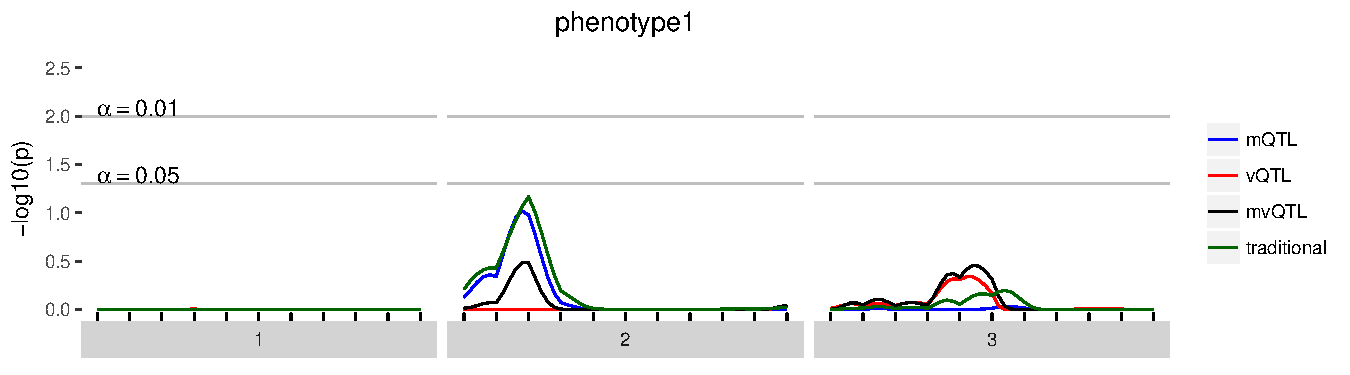
\includegraphics[width=\textwidth]{images/empir_p_scan_phenotype1.pdf}
    \end{subfigure}

    \begin{subfigure}[b]{0.9\textwidth}
        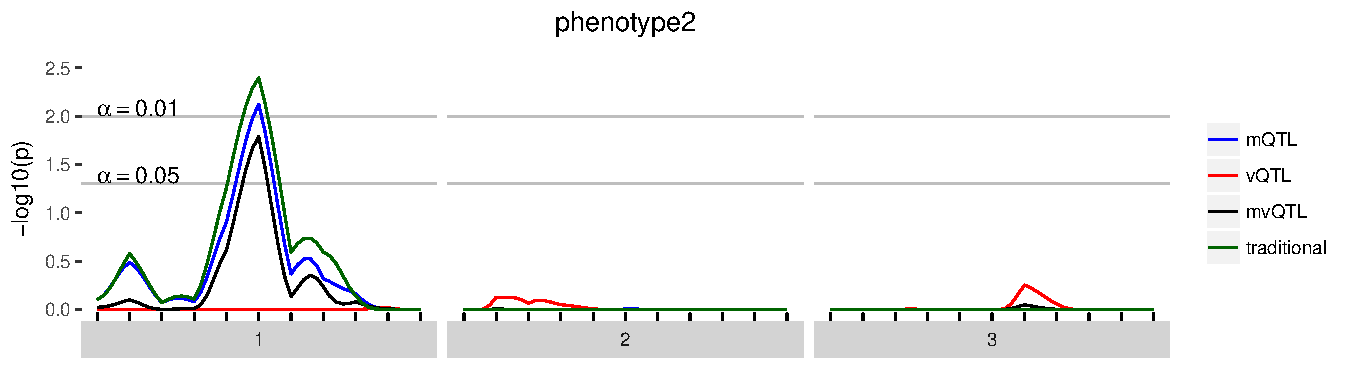
\includegraphics[width=\textwidth]{images/empir_p_scan_phenotype2.pdf}
    \end{subfigure}

    \begin{subfigure}[b]{0.9\textwidth}
        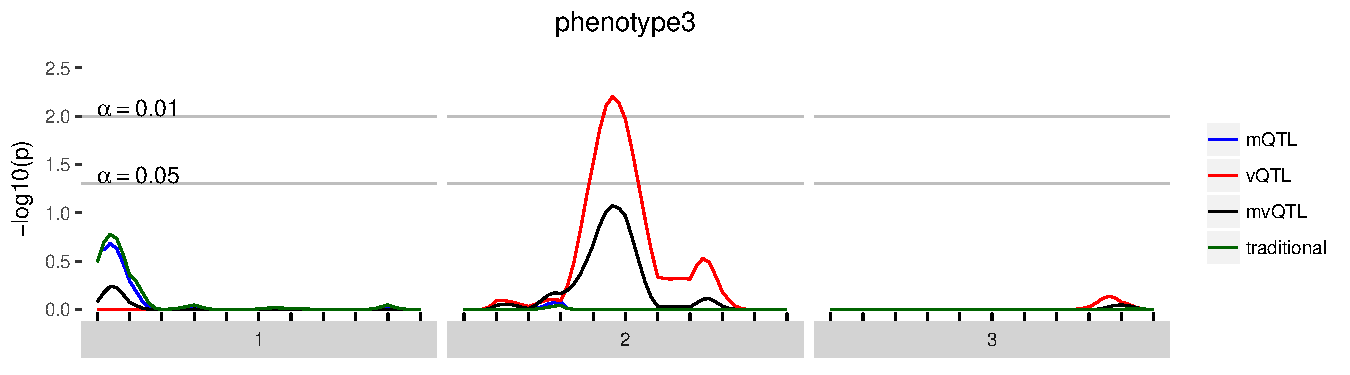
\includegraphics[width=\textwidth]{images/empir_p_scan_phenotype3.pdf}
    \end{subfigure}

    \begin{subfigure}[b]{0.9\textwidth}
        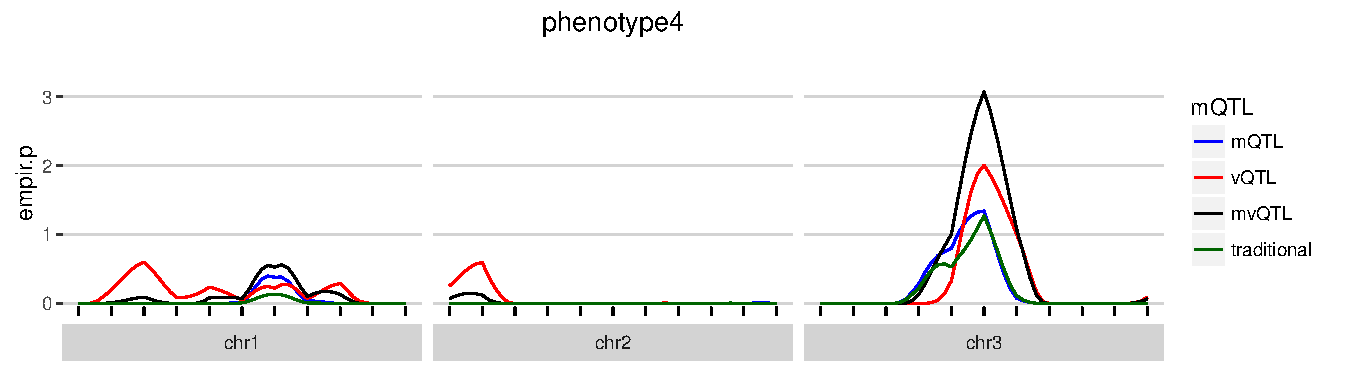
\includegraphics[width=\textwidth]{images/empir_p_scan_phenotype4.pdf}
    \end{subfigure}

    \caption{For each of the four simulated phenotypes, the genome scan shows the -log10 of the FWER-corrected $p$-value of each test -- mean, variance, and joint -- in blue, red, and black, respectively. Thus, a value of 3 implies that the quantity of evidence against the null is such that we expect to see this much or more evidence once per thousand genome scans when there is no true effect. \label{fig:empir_p_scans}}
\end{figure}

The $p$-value assigned to each locus by calculating the position of its calculated LOD score in its null distribution answers the question, ``How probable is it to observe this much of a deviation from the null at this locus, given that there is no true effect?''
This question is not entirely relevant for genetic mapping, however, because we typically test for association at many loci, with no special interest in any individual locus \textit{a priori}.
Thus, a more appropriate $p$-value would answer the question, ``How probable is it to observe this much or more deviation from the null at \textit{some} locus in the genome, given that there are no true effects?''
This is precisely the reasoning behind the family-wide-error-rate (FWER) controlling procedure we illustrate below.

To calculate a FWER-controlling $p$-value, one typically must estimate the effective number of statistical tests conducted.
The effective number of tests in a genome scan, however, is difficult to estimate.
One lower bound is the number of chromosomes.
Due to the randomization in meiosis no two non-syntenic loci are correlated in an experimental cross and therefore tests on different chromosomes are always independent.
But there are many non-identical tests conducted on each chromosome, so the number of chromosomes is an under-estimate.
One upper bound on the effective number of tests is the total number of loci.
But, loci on the same chromosome are often in linkage disequilibrium, therefore the tests are not independent and the total number of loci is an over-estimate \citep{Lander1989a}.

Like previous work on permutation-based thresholds for genetic mapping \citep{Churchill1994,Carlborg2002}, our permutation approach sidesteps estimation of the effective number of tests.
We conduct many permuted genomes scans, each executing a carefully-constructed model comparison to maintain all mean and variance effects of covariates and any non-focal genetic effects on mean and variance.
The details of these model comparisons are provided in the companion article [Corty2017a].
For each test, we extract the highest observed value of the test statistic from each permutation scan and use those to model a generalized extreme value (GEV) density \citep{Stephenson2002}.
The observed LOD scores from the genome scan are then transformed by the cumulative distribution function of the extreme value density to estimate the FWER-controlling $p$-values.
This approach is implemented in the function, \texttt{scanonevar.perm}, which requires two inputs:

\begin{enumerate}
	\item \texttt{sov} is the \texttt{scanonevar} object, the statistical significance of which will be assessed through permutation.
	\item \texttt{n.perms} is the number of permutations to conduct.
\end{enumerate}

The object returned by \texttt{scanonevar.perm} is a \texttt{scanonevar} object with one important additional piece of information, an empirical $p$-value for each test at each locus.
These $p$-values are FWER-corrected, so a value of $0.05$ for a specific test at a specific locus implies that in 5\% of similar experiments where there is no true genotype-phenotype association, we would expect to observe \textit{some} locus with this much or more evidence of association.
Additionally, the returned object contains a list of the per-genome-scan maximum observed LOD for each test and each chromosome type.

Accurate estimation of the FWER-controlled $p$-values requires many permutation scans.
We recommend at least 100, and rarely more than 1000 \citep{Churchill1994,Carlborg2002}.
These permutation scans can be run on multiple processors by specifying the optional \texttt{n.cores} argument, which defaults to the total number of cores on the computer minus 2.
On an Intel Core i5, running 100 permutations on this dataset packtakes about five minutes.
When many phenotypes are studied, or if faster runtimes are needed, these permutation scans can be broken into groups with different values for \texttt{random.seed}, run on separate computers, and combined with the \texttt{c} function.
This function combines the permutations from all the inputted scans, re-evaluates the observed LOD scores in the context of all available permutations, and returns a new \texttt{scanonevar} object with more precisely estimated empirical $p$-values.




\section*{Investigate Significant Findings}

\begin{figure}[ht]
    \begin{subfigure}[t]{0.5\textwidth}
        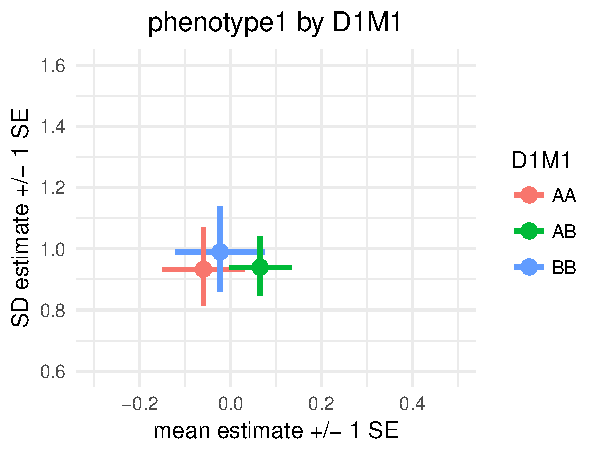
\includegraphics[width=\textwidth]{images/mean_var_plot_phen1.pdf}
    \end{subfigure}
    \hfill
    \begin{subfigure}[t]{0.5\textwidth}
        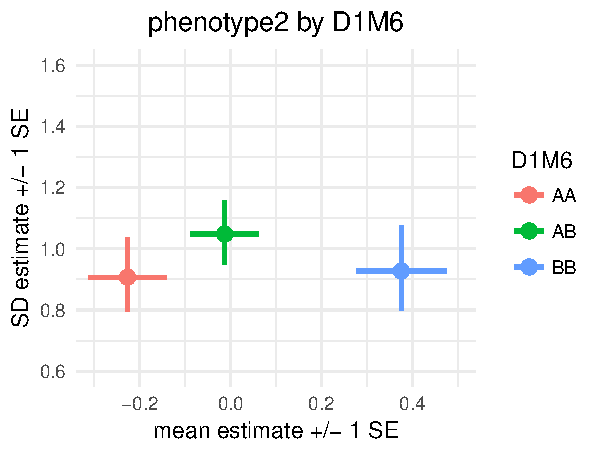
\includegraphics[width=\textwidth]{images/mean_var_plot_phen2.pdf}
    \end{subfigure}

    \begin{subfigure}[t]{0.5\textwidth}
        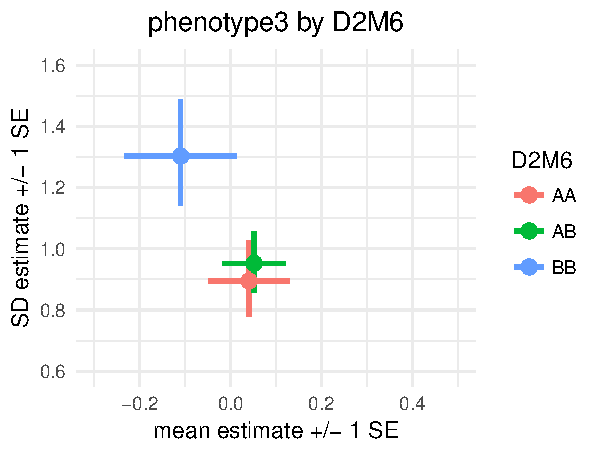
\includegraphics[width=\textwidth]{images/mean_var_plot_phen3.pdf}
    \end{subfigure}
    \hfill
    \begin{subfigure}[t]{0.5\textwidth}
        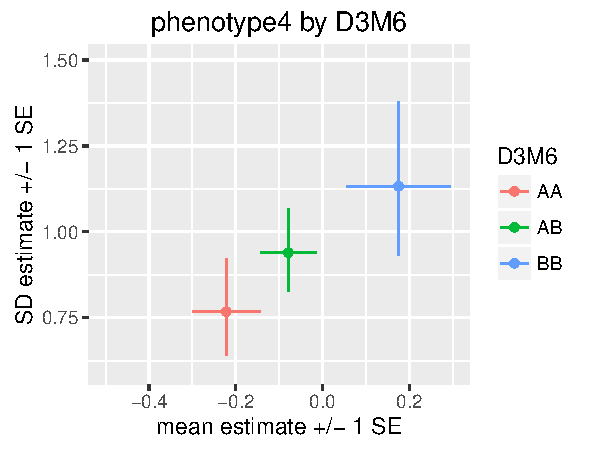
\includegraphics[width=\textwidth]{images/mean_var_plot_phen4.pdf}
    \end{subfigure}

    \caption{\texttt{mean\_var\_plot}s show the estimated genotype effects at a locus, with mean effects on the horizontal axis and variance effects on the vertical axis.  Horizontal lines indicate standard errors for mean effects and vertical lines indicate standard errors for variance effects.  More information on the interpretation of these plots is provided in the `Investigate Significant Findings' section. \label{fig:mean_var_plots}}
\end{figure}

Having identified some QTL, we want to visualize the estimated genetic and covariate effects at the QTL.
Because the \texttt{vqtl} package models both mean and variance effects, existing plotting utilities aren't able to display the entirety of the modeling results.
To investigate the results of a \texttt{vqtl} scan at one particular locus, we developed the \texttt{mean\_var\_plot}.
This plot shows information about the phenotype mean on the horizontal axis and information about the phenotype variance on the vertical axis.
There are both ``model-free'' and ``model-based'' versions of this plotting utility.
Here we show only the ``model-based'' version.

Figure~\ref{fig:mean_var_plots} shows a model-based \texttt{mean\_var\_plot} for each of the four phenotypes.
In each plot, the location of the dot shows the estimated mean and standard deviation of each genotype group, with the mean indicated by the horizontal position and the standard deviation indicated by the vertical position.
The horizontal lines extending to the left and right from each dot show the standard error of the mean estimate, and the vertical lines extending up and down from each dot show the standard error of the standard deviation estimate.
There are two types of grouping factors considered by the function \texttt{mean\_var\_plot\_model\_based}:
(1) \texttt{focal.groups} are groups that are modeled and the prediction for each group is plotted.
For example, a genetic marker is the \texttt{focal.group} in each plot in figure~\ref{fig:mean_var_plots}; \texttt{D1M1} in the top left, \texttt{D1M6} in the top right, etc.
(2) \texttt{nuisance.groups} are groups that are modeled, but then averaged over before plotting.
When there are many grouping factors thought to play a role in determining the mean and variance of an individual's phenotype, such as sex, treatment, and batch, we recommend putting just one or two in \texttt{focal.groups} and the others in \texttt{nuisance.groups} for clarity, cycling through which are displayed to gain a thorough understanding of the factors that determine the mean and variance of the phenotype.

For \texttt{phenotype1}, the \texttt{mean\_var\_plot} is shown at the first marker of the first chromosome.
The estimates of the genotype effects on phenotype mean and variance are within one standard error of each other.
This pattern is consistent with the fact that there are no genetic effects, and the $p$-value was not statistically significant at any locus.

For \texttt{phenotype2}, the \texttt{mean\_var\_plot} is shown at the most significant marker, the sixth marker on the first chromosome.
The estimates of the genotype effects differ in the horizontal axis, but not the vertical axis.
This pattern is consistent with the fact that there is a genetic effect on phenotype mean but none on phenotype variance and with the highly significant $p$-value for the mQTL test, but non-significant $p$-value for the vQTL test.

For \texttt{phenotype3}, the \texttt{mean\_var\_plot} is shown at the most significant marker, the sixth marker on the second chromosome.
The estimates of the genotype effects differ in the vertical axis, but on on the horizontal axis.
This pattern is consistent with the fact that there is a genetic effect on phenotype variance but none on phenotype mean and with the highly significant $p$-value for the vQTL test but non-significant $p$-value for the mQTL test.

For \texttt{phenotype4}, the \texttt{mean\_var\_plot} is shown at the most significant marker, the sixth marker on the third chromosome.
The estimates fo the genotype effects differ somewhat in both the horizontal and vertical axes, but not as much on the horizontal axis as \texttt{phenotype2} and not as much on the vertical axis as \texttt{phenotype3}.
This pattern is consistent with the fact that there is a genetic effect on both phenotype mean and variance and with the highly significant $p$-value for the mvQTL test and the marginally significant $p$-values for the other two tests.

Additional plotting utilities, \texttt{phenotype\_plot}, \texttt{effects\_plot} and \texttt{mean\_var\_plot\_model\_free} are described in the online vignette for the \texttt{vqtl} package, available at \texttt{github.com/rcorty}.


Finally, it is important to assess the genetic precision of a discovered QTL.
This step allows for bioinformatic follow-up.
The function \texttt{scanonevar.boot} implements the non-parametric and Bayesian bootstrap.
This function takes, as arguments, a \texttt{scanonevar} object, the name of the chromosome containing the QTL, and \texttt{num.resamples}, the number of bootstrap resamplings desired.

In our experience, 1000 resamples is an appropriate number to establish 80\% and 90\% confidence intervals.
With the datasets simulated here, it takes 15 minutes to run 500 bootstrap resamples on an Intel core i5.

% \section*{Mathematical Details}

% [todo]

% mean-var plot what is on x what is on y and how are SE's calculated

% DGLM with other links and distribs


\section*{Conclusion}

We have demonstrated typical usage of the \texttt{vqtl} \texttt{R} package for QTL mapping in experimental crosses.
This package is most appropriate for crosses and phenotypes where nuisance covariates or genetic factors are known or suspected to influence phenotype variance.
In the case of genetic factors, they can be mapped.
In the case of nuisance covariates, they can be accommodated.

The central function of this package, \texttt{scanonevar}, carries out the initial genome scan.
The permutation function, \texttt{scanonevar.perm}, executes a set of permutations to empirically estimate a FWER-controlling $p$-value for each observed LOD score.
A suite of plotting functions, e.g. the \texttt{mean\_var\_plot}, allows geneticists to evaluate the allelic and covariate effects that underlie detected signals.
The bootstrap function, \texttt{scanonevar.boot}, executes bootstrap resampling to assess the genetic precision of a QTL and extablish a confidence interval. 


\printbibliography


\clearpage
\newpage
\section*{Appendix}

\begin{figure}[ht!]
    \begin{subfigure}[b]{0.9\textwidth}
        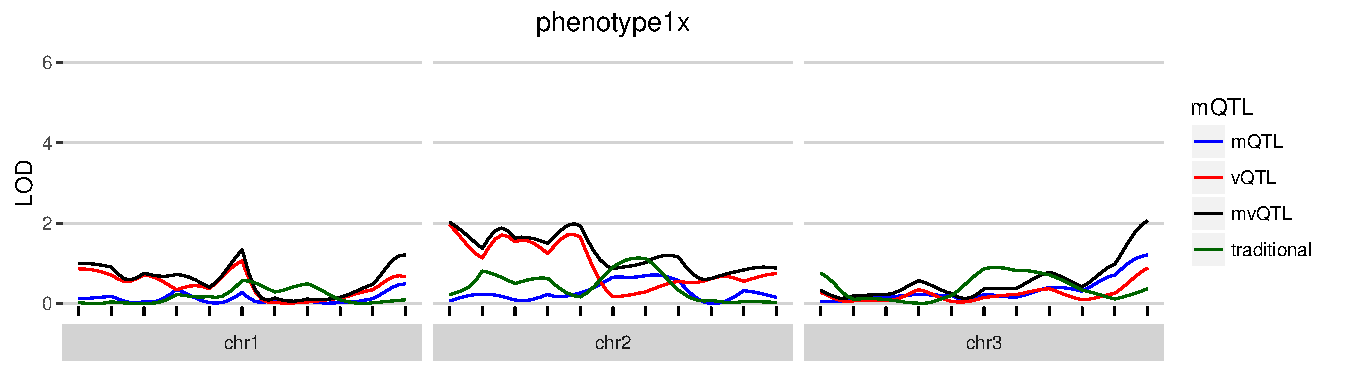
\includegraphics[width=\textwidth]{images/LOD_scan_phenotype1x.pdf}
    \end{subfigure}

    \begin{subfigure}[b]{0.9\textwidth}
        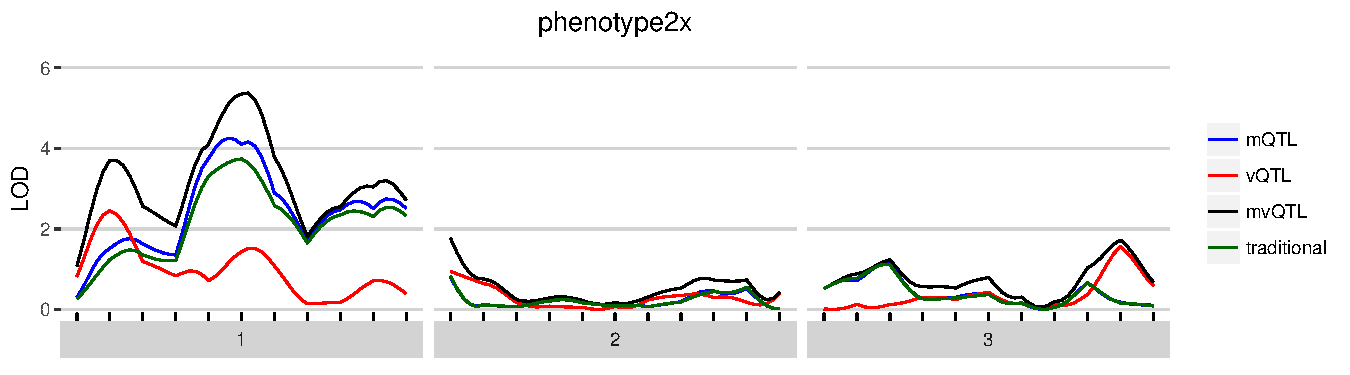
\includegraphics[width=\textwidth]{images/LOD_scan_phenotype2x.pdf}
    \end{subfigure}

    \begin{subfigure}[b]{0.9\textwidth}
        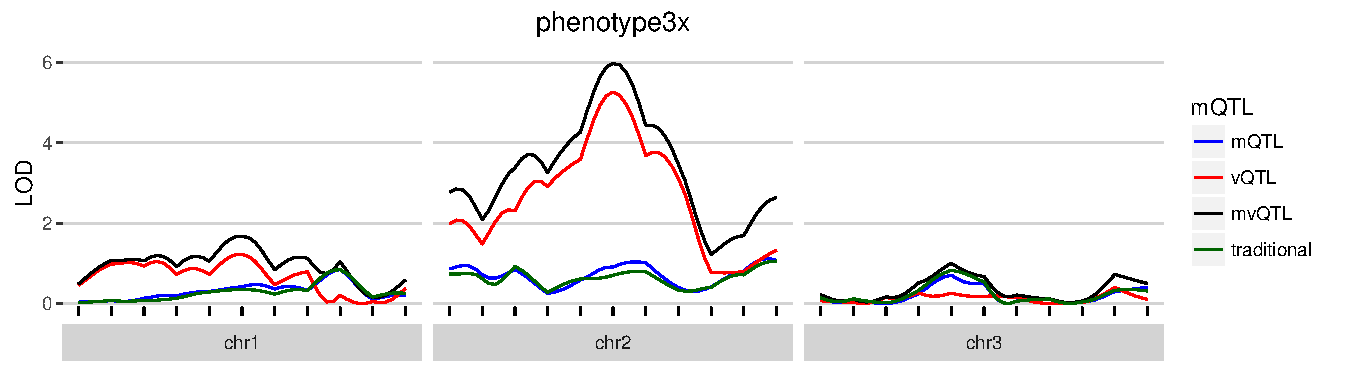
\includegraphics[width=\textwidth]{images/LOD_scan_phenotype3x.pdf}
    \end{subfigure}

    \begin{subfigure}[b]{0.9\textwidth}
        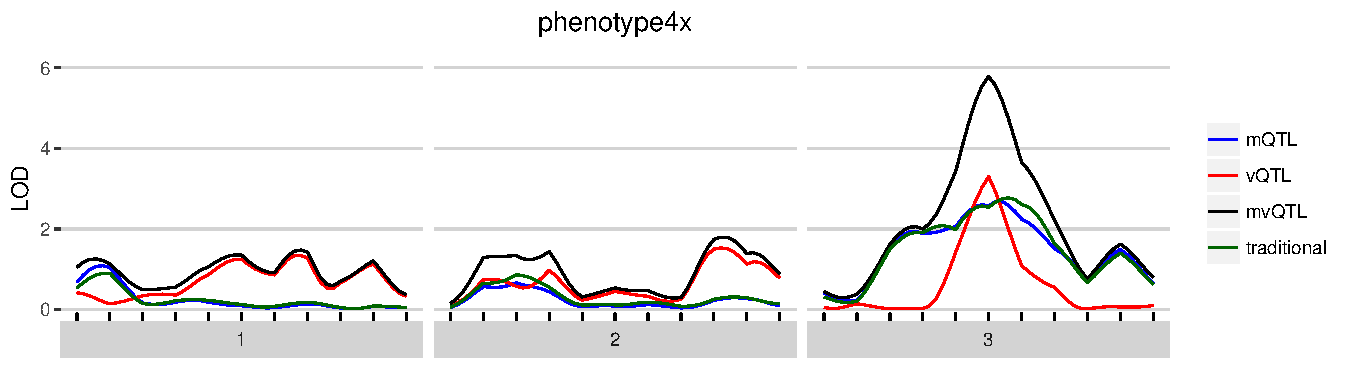
\includegraphics[width=\textwidth]{images/LOD_scan_phenotype4x.pdf}
    \end{subfigure}

    \caption{For each of the four simulated phenotypes, the genome scan shows the LOD score of each test -- mean, variance, and joint -- in blue, red, and black, respectively.  The traditional test is in green and globally similar to the mean test. \label{fig:apdx_lod_score_scans}}
\end{figure}



\begin{figure}[ht!]
    \begin{subfigure}[b]{0.9\textwidth}
        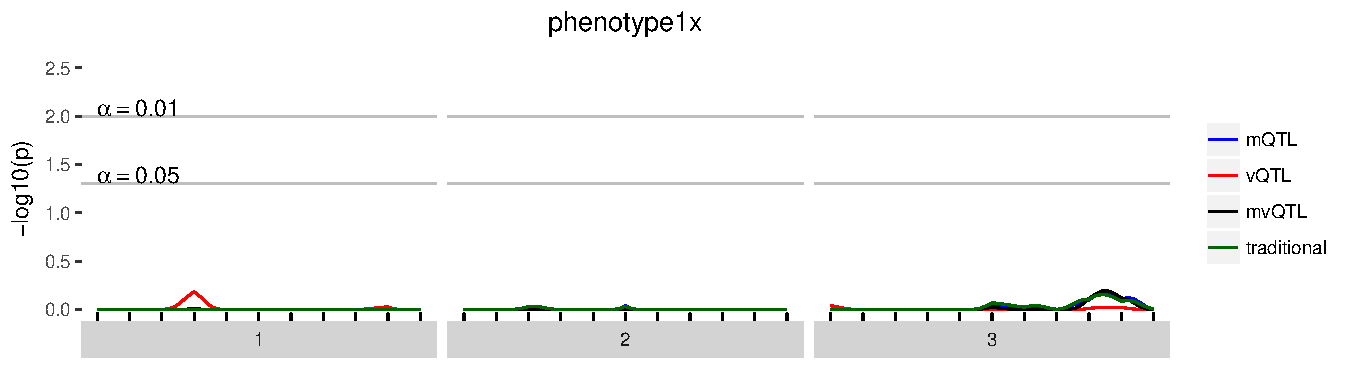
\includegraphics[width=\textwidth]{images/empir_p_scan_phenotype1x.pdf}
    \end{subfigure}

    \begin{subfigure}[b]{0.9\textwidth}
        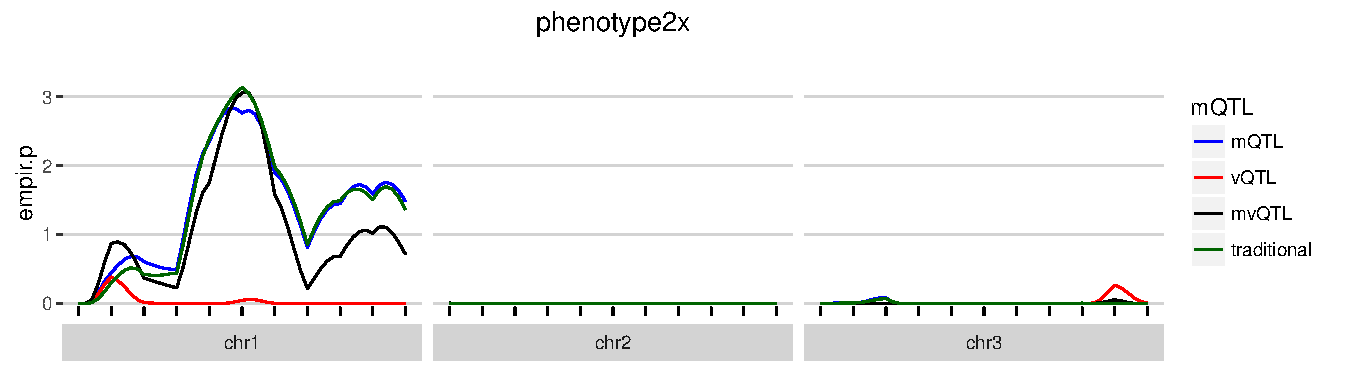
\includegraphics[width=\textwidth]{images/empir_p_scan_phenotype2x.pdf}
    \end{subfigure}

    \begin{subfigure}[b]{0.9\textwidth}
        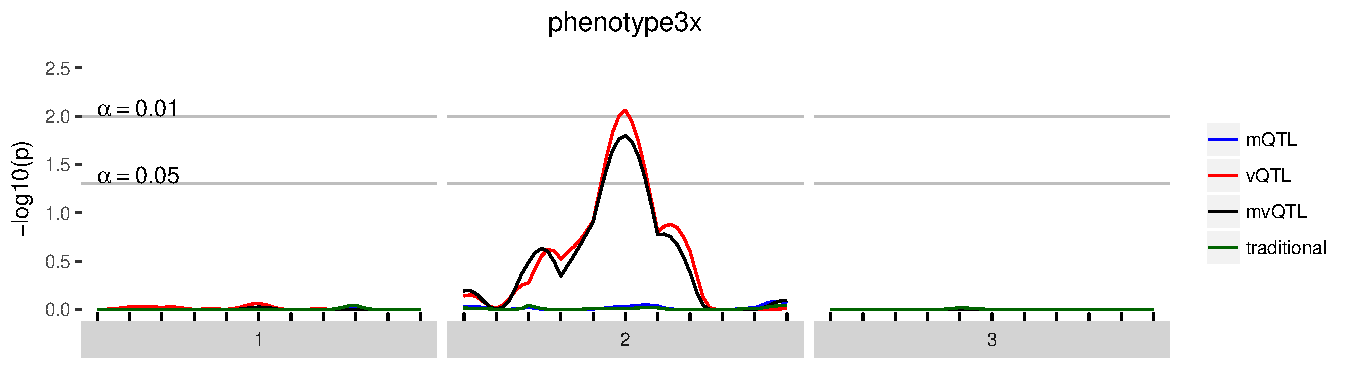
\includegraphics[width=\textwidth]{images/empir_p_scan_phenotype3x.pdf}
    \end{subfigure}

    \begin{subfigure}[b]{0.9\textwidth}
        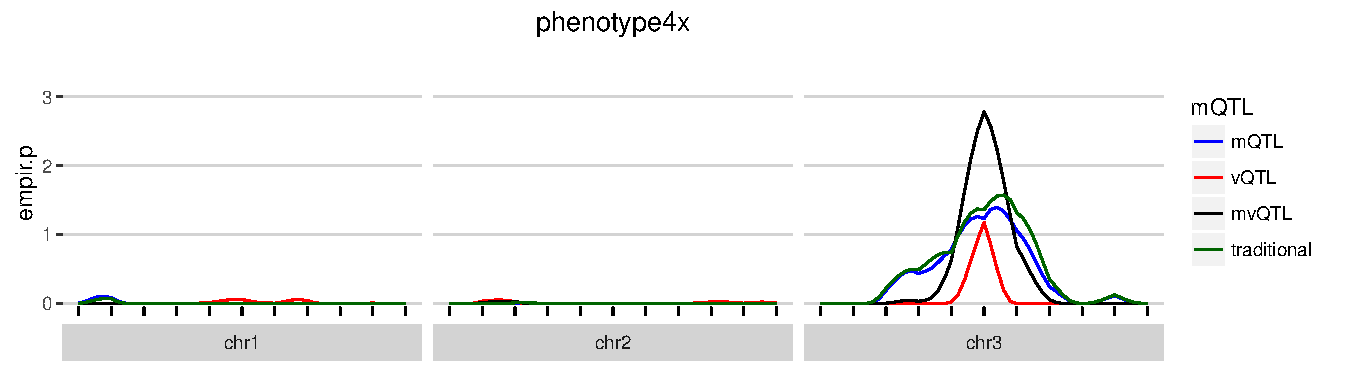
\includegraphics[width=\textwidth]{images/empir_p_scan_phenotype4x.pdf}
    \end{subfigure}

    \caption{For each of the four simulated phenotypes, the genome scan shows the -log10 of the FWER-corrected $p$-value of each test -- mean, variance, and joint -- in blue, red, and black, respectively. Thus, a value of 3 implies that the quantity of evidence against the null is such that we expect to see this much or more evidence once per thousand genome scans when there is no true effect. \label{fig:apdx_empir_p_scans}}
\end{figure}


\begin{figure}[htbp]
    \begin{subfigure}[t]{0.5\textwidth}
        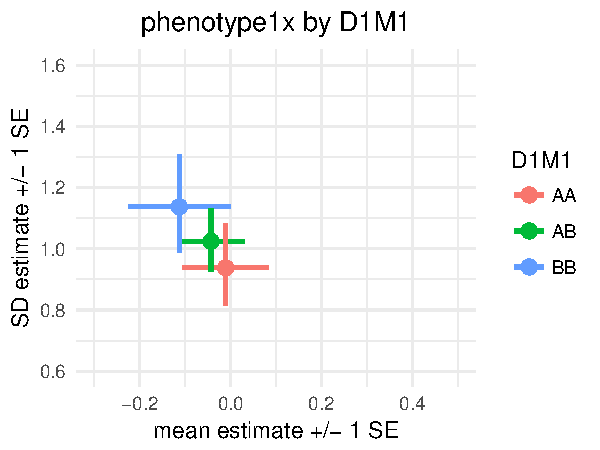
\includegraphics[width=\textwidth]{images/mean_var_plot_phen1x.pdf}
    \end{subfigure}
    \hfill
    \begin{subfigure}[t]{0.5\textwidth}
        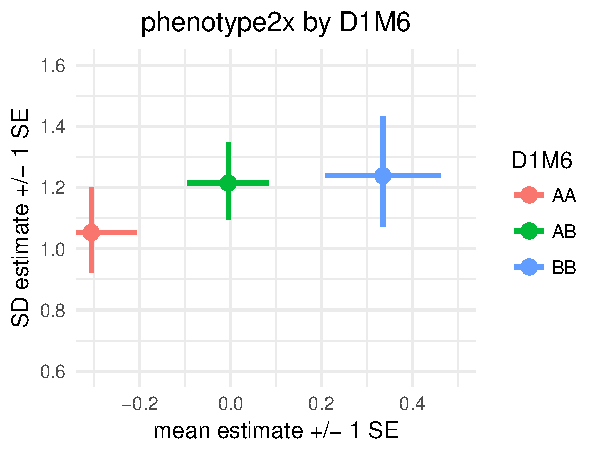
\includegraphics[width=\textwidth]{images/mean_var_plot_phen2x.pdf}
    \end{subfigure}

    \begin{subfigure}[t]{0.5\textwidth}
        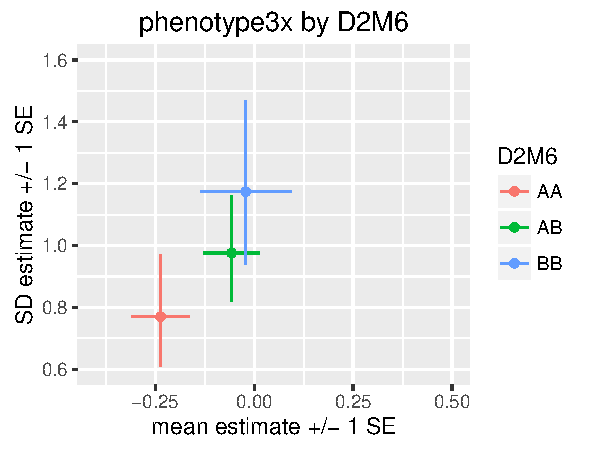
\includegraphics[width=\textwidth]{images/mean_var_plot_phen3x.pdf}
    \end{subfigure}
    \hfill
    \begin{subfigure}[t]{0.5\textwidth}
        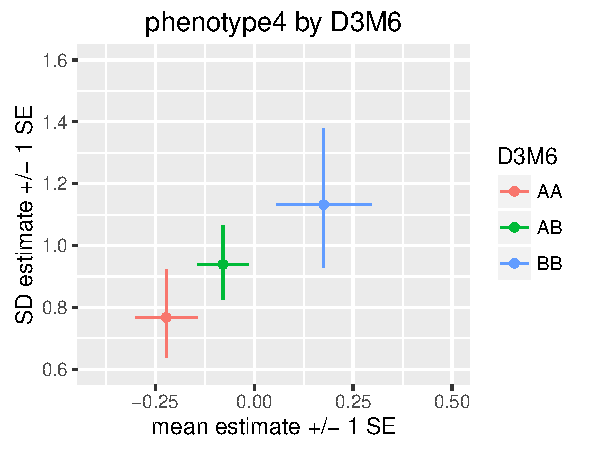
\includegraphics[width=\textwidth]{images/mean_var_plot_phen4x.pdf}
    \end{subfigure}

    \caption{\texttt{mean\_var\_plot}s show the estimated genotype effects at a locus, with mean effects on the horizontal axis and variance effects on the vertical axis.  Horizontal lines indicate standard errors for mean effects and vertical lines indicate standard errors for variance effects.  More information on the interpretation of these plots is provided in the `Investigate Significant Findings' section. \label{fig:apdx_mean_var_plots}}
\end{figure}

\end{document}